\documentclass[a4paper]{article}

\usepackage[english]{babel}
\usepackage[utf8]{inputenc}
\usepackage{caption}
\usepackage{fancyhdr}
\usepackage{float}
\usepackage{listings}
\usepackage{pgfplots}
\usepackage{vmargin}
\usepackage{wrapfig}

% ------------------------------------------------------------------------------
% general
% ------------------------------------------------------------------------------
\setpapersize{A4}
\setmargins
  {2.5cm}{2.0cm}  % left and top margin
  {16cm}{22cm}    % text width and height
  {48pt}{36pt}    % header height and spacing
  {0pt}{30pt}     % footer height and spacing

\pagestyle{fancy}

\sloppy
\frenchspacing

\setlength{\parindent}{0pt}
\setlength{\parskip}{5pt}
\setlength{\fboxsep}{1.5mm}

% ------------------------------------------------------------------------------
% colors
% ------------------------------------------------------------------------------
% \definecolor{codegreen}{rgb}{0,0.6,0}
% \definecolor{codegray}{rgb}{0.5,0.5,0.5}
% \definecolor{codepurple}{rgb}{0.38,0,0.72}

% ------------------------------------------------------------------------------
% commands
% ------------------------------------------------------------------------------
\newcommand{\ceil}[1]{\left\lceil{} {#1} \right\rceil{}}
\newcommand{\floor}[1]{\left\lfloor{} {#1} \right\rfloor{}}

% ------------------------------------------------------------------------------
% `pgfplots` setup
% ------------------------------------------------------------------------------
\pgfplotsset{compat=1.18}

\usepgfplotslibrary{
  dateplot,
  statistics,
}

% ------------------------------------------------------------------------------
% `listings` setup
% ------------------------------------------------------------------------------
\lstset{
  numbers=none,
  basicstyle=\ttfamily,
  upquote=true,
}


\begin{document}
\lhead{
  \begin{tabular}{l}
    {\bf Decentralized Systems: IPFS Lab Report}\\
    {\bf Submitted by:} Maxim Rastorguev, Roman Popa
  \end{tabular}
}
\rhead{}


\section{Basic ideas of IPFS}

% https://docs.ipfs.tech/concepts/file-systems/#unix-file-system-unixfs
% ipfs add --help
% ipfs cat --help
\subsection{File upload, download and storage}

A file can be uploaded to IPFS by issuing \verb|ipfs add PATH...| on the
command line. The \verb|ipfs add| command is handled in
\verb|kubo/core/commands/add.go|, which later delegates everything to
\verb|UnixfsAPI.Add()|. There the file is split into smaller parts called
chunks, if necessary, and a CID is computed for every chunk. If the file is
small enough, only one chunk will be created. Additionally, layouting is
performed: file chunks are arranged into a Merkle DAG and uploaded. Metadata
about the chunks is stored in a UnixFS node. There are two strategies for
building the Merkle DAG: \verb|balanced| (default) and \verb|trickle|. When the
upload for all chunks is done, the CID of the root of the DAG is returned to
the user as a reference to the file.

A file can be downloaded from IPFS by issuing \verb|ipfs cat IPFS-PATH...| on
the command line. The CID is used to lookup the content in the DHT and find
IPFS instances that store the content linked by the CID. When downloading a
file, the Merkle DAG is traversed in in-order and the content of every chunk is
sent back. It is also possible to read only a particular byte range from the
file by specifying the offset and length.


\subsection{Peer connections}

Kubo has a hardcoded list of bootstrap nodes
(\verb|go-libp2p-kad-dht/dht_bootstrap.go| and
\verb|config/bootstrap_peers.go|). When launched, it will try to automatically
connect to them and fill its routing table with peers. From time to time (10
minutes by default), it will evict peers if not reachable
(\verb|go-libp2p-kad-dht/rtrefresh/rt_refresh_manager.go|). If an IPFS instance
is encountered while querying (\verb|go-libp2p-kad-dht/query.go| -
\verb|IpfsDHT.runQuery()|), Kubo will check if it is eligible to be added to
the routing table and add it (\verb|go-libp2p-kad-dht/dht.go| -
\verb|IpfsDHT.rtPeerLoop()|).


\section{Implementation}

The code is organized in two repositories:
\begin{itemize}
\item https://github.com/x4204/rptu-dec-sys-ws24-kubo - this repository
contains the modified source code of Kubo. All code changes can be found on
branch \verb|dec-sys|
\item https://github.com/x4204/rptu-dec-sys-ws24 - this repository contains
everything else related to the lab itself: deployment, benchmark and metric
gathering scripts as well as documentation on how to setup and run them
\end{itemize}

\textbf{Code changes.}\\
The following modifications were made to the source code of Kubo:
\begin{itemize}
\item remove hardcoded lists of bootstrap addresses in
\verb|config/bootstrap_peers.go| and \verb|go-libp2p-kad-dht/dht_bootstrap.go|.
Done because we don't want Kubo to automatically connect to them
\item disable MDNS in \verb|config/init.go|. Done, because it is hardcoded to
\verb|true| and ignores the config option \verb|Discovery.MDNS.Enabled|
\item disable \verb|dht.rtRefreshManager|, \verb|dht.rtPeerLoop()| and
\verb|dht.runFixLowPeersLoop()| in \verb|go-libp2p-kad-dht/dht.go|. These
places are responsible for triggering peer lookup and adding peers to the
routing table if any new ones were encountered while running queries
\end{itemize}

\textbf{Config changes.}\\
Docker compose is used to run an IPFS swarm. The following swarm key is mapped
into every container:
\begin{lstlisting}
/key/swarm/psk/1.0.0/
/base16/
3ffe35d22f310d2505b21a1b104f23d9e19534ae0a610d8717eada1d79e4f9b8
\end{lstlisting}

Additionally, the following commands run before the container starts:
\begin{lstlisting}
ipfs config --json Bootstrap '[]'
ipfs config --json Routing.Type '"dht"'
ipfs config --json Discovery.MDNS.Enabled 'false'
\end{lstlisting}

The first command removes all bootstrap nodes from the config file. The second
command configures Kubo to use \verb|dht| routing, which is required by Kubo
when running in swarm mode. Finally, with the third command we explicitly
disable mDNS for peer lookup in local network.

As an additional measure, we also set the environment variable
\verb|LIBP2P_FORCE_PNET=1| to force the usage of private networks, as suggested
in the documentation.

\textbf{Peer behaviour simulation.}\\
The deployment of any specific topology is automated
\footnote{https://github.com/x4204/rptu-dec-sys-ws24/blob/master/deploy/main.py}
and is capable of deploying nodes and linking them according to a given config
file as well visualising it. Topology files are just a list of nodes and links
between them, for example:
\begin{lstlisting}
nodes = [
  'ipfs-00',
  'ipfs-01',
  'ipfs-02',
]

links = [
  ['ipfs-00', 'ipfs-01'],
  ['ipfs-01', 'ipfs-02'],
]
\end{lstlisting}

\textcolor{red}{
  \textbf{TODO:} Then, you should elaborate on how you simulate the behaviors
  of peers, the setup of simulations, and the simulated topologies.
}


\section{Results}

\textcolor{red}{
  \textbf{TODO:} You need to display your results in a clear and understandable
  way with concrete numbers. Based on the results and profiles you obtained
  from simulations, you need to compare the performance of different topologies
  and explain the differences. Then, you need to discuss which topologies
  result in benefits to network performance.
}

\textbf{Benchmarking methodology}\\
In every test the entire topology is recreated and the storage is wiped to
ensure a clean state. Container metrics are collected using docker stats. File
sizes take values from \verb|1 MiB| to \verb|500 MiB| and follow the zipf
distribution with parameter $a=1.5$. The content of the files is randomly
generated using \verb|/dev/urandom| device as a source for randomness. The
benchmark runs for 5 minutes with 100 concurrent clients and a 85/15 read/write
workload. Nodes are chosen uniformly at random for upload/download.

\textcolor{red}{\textbf{TODO: compute average for every usecase and metric}}\\

\subsection{\textcolor{red}{Case 1: Kubo without source code modifications}}

\begin{figure}[H]
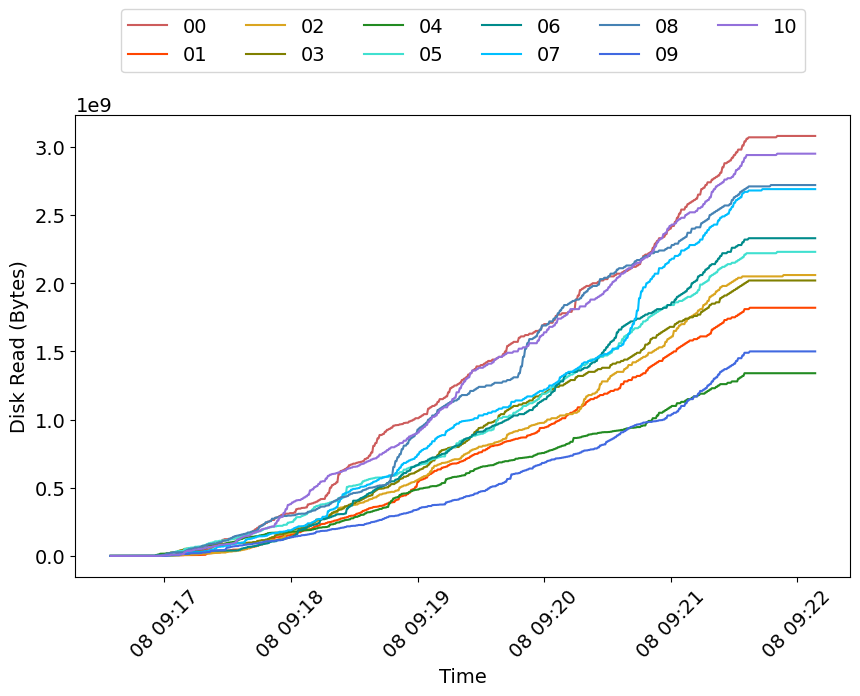
\includegraphics[width=\linewidth]{figures/original/blk_read.png}
\caption{Original Kubo -- amount of bytes read from disk}
\end{figure}
\begin{figure}[H]
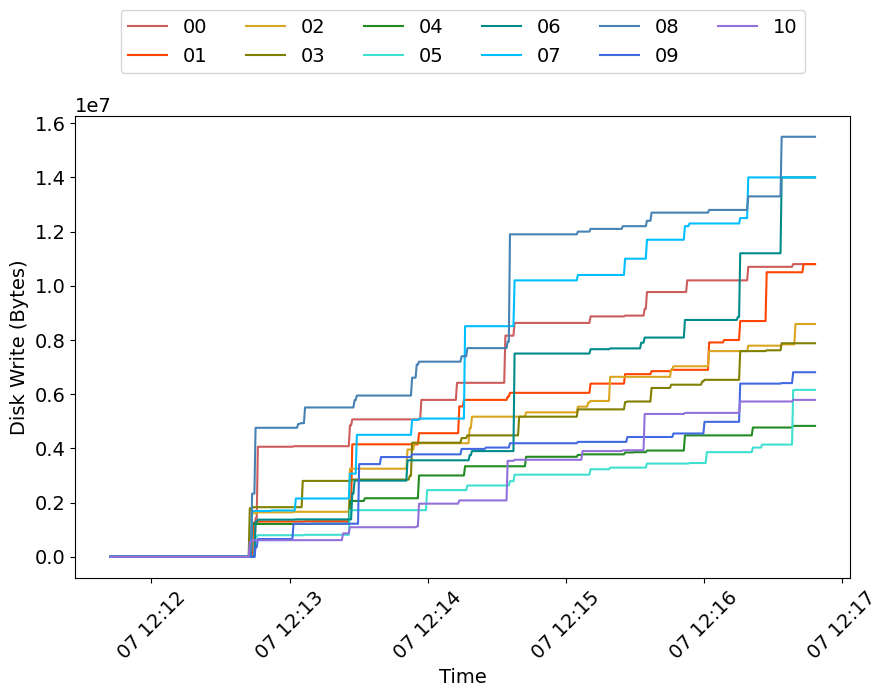
\includegraphics[width=\linewidth]{figures/original/blk_write.png}
\caption{Original Kubo -- amount of bytes written to disk}
\end{figure}
\begin{figure}[H]
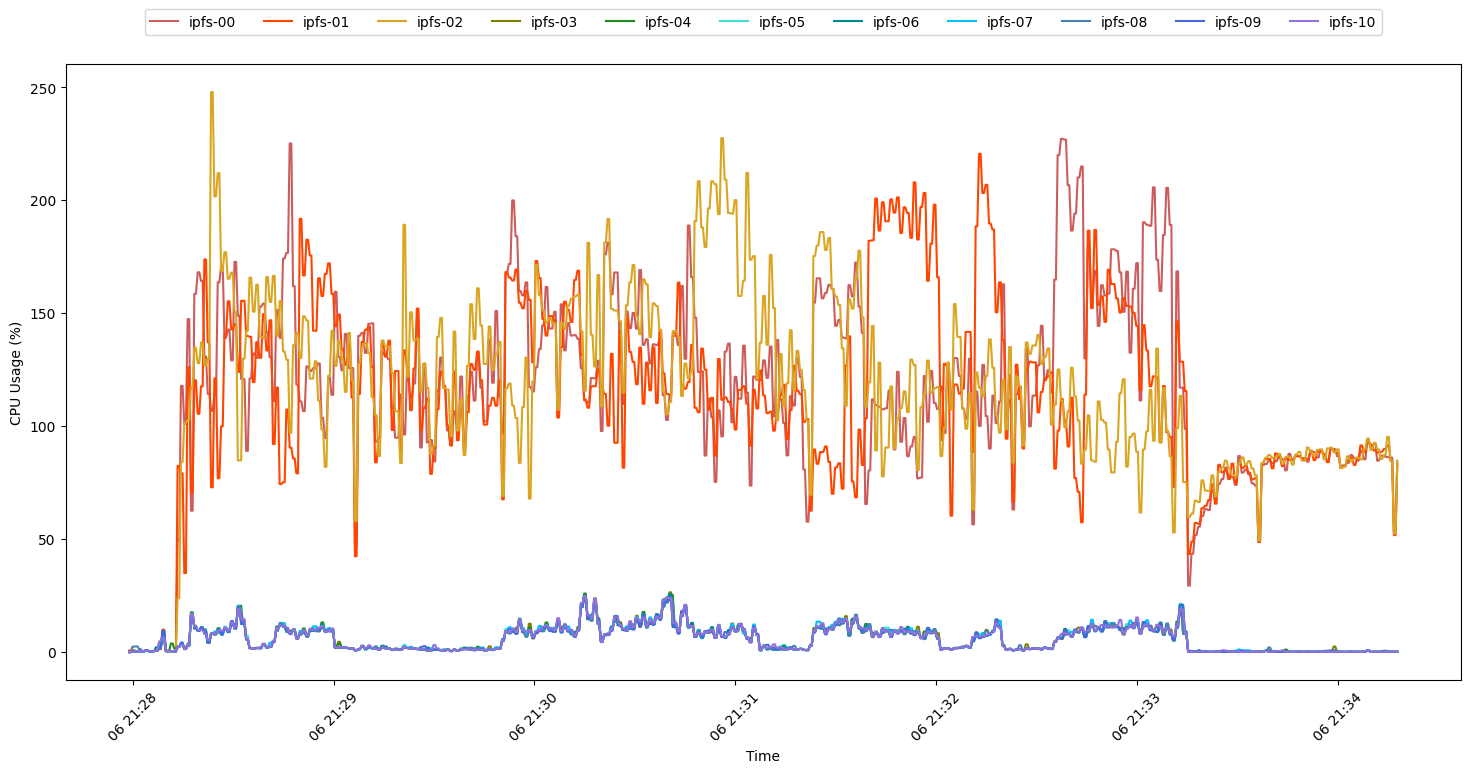
\includegraphics[width=\linewidth]{figures/original/cpu_usage.png}
\caption{Original Kubo -- CPU usage}
\end{figure}
\begin{figure}[H]
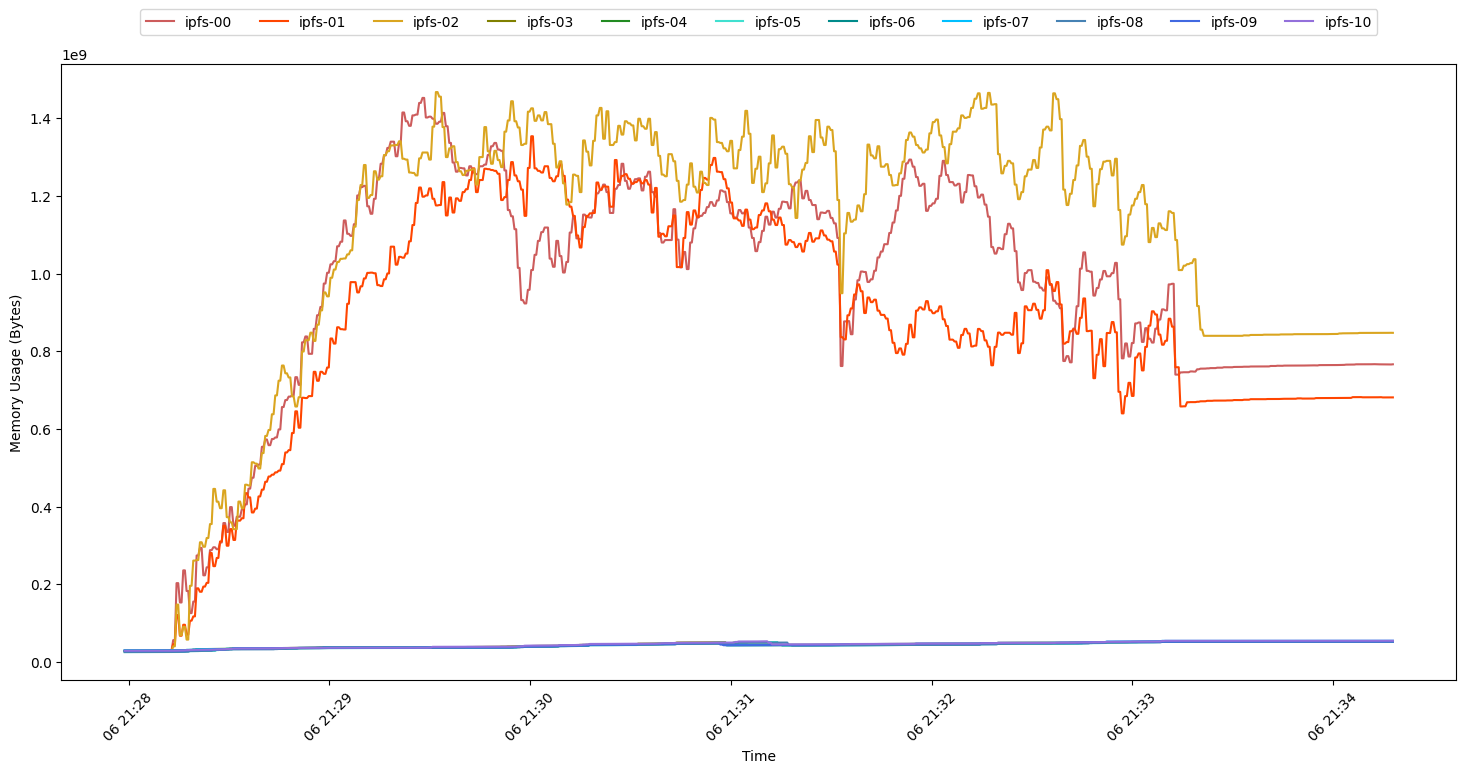
\includegraphics[width=\linewidth]{figures/original/mem_usage.png}
\caption{Original Kubo -- memory usage}
\end{figure}
\begin{figure}[H]
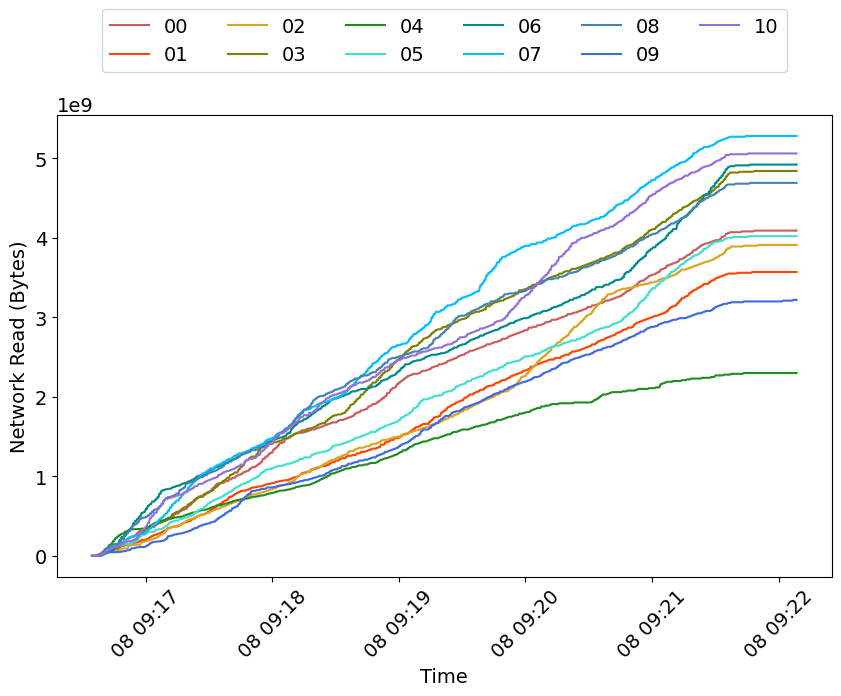
\includegraphics[width=\linewidth]{figures/original/net_read.png}
\caption{Original Kubo -- amount of bytes received over network}
\end{figure}
\begin{figure}[H]
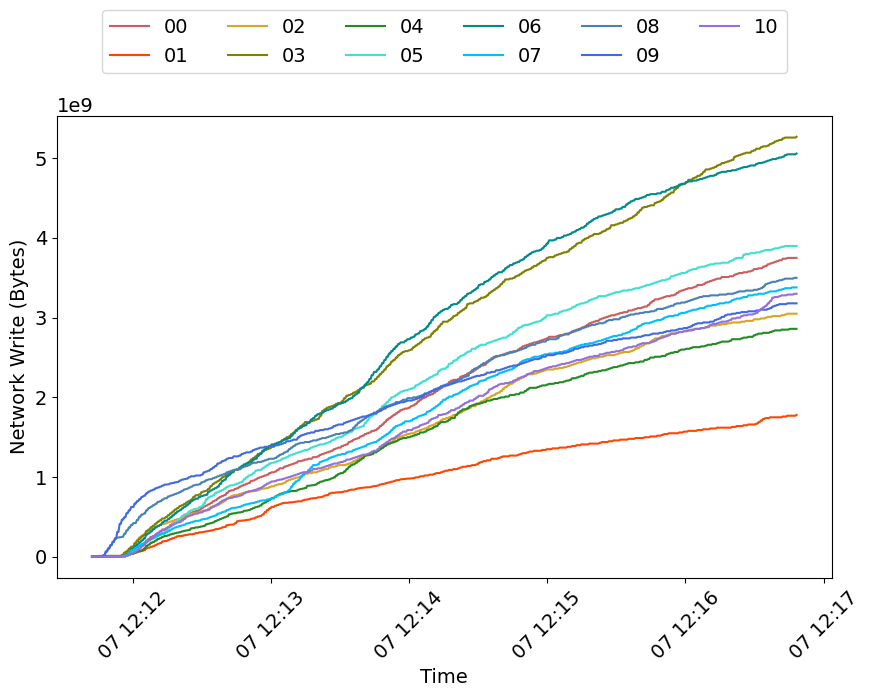
\includegraphics[width=\linewidth]{figures/original/net_write.png}
\caption{Original Kubo -- amount of bytes transmitted over network}
\end{figure}


\subsection{\textcolor{red}{Case 2: Ring Topology}}

\begin{figure}[H]
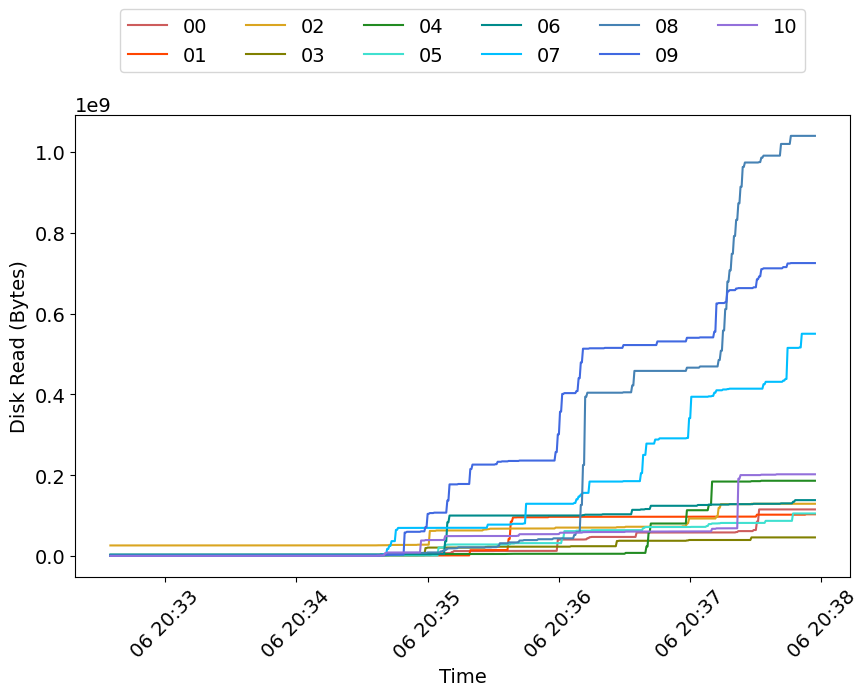
\includegraphics[width=\linewidth]{figures/ring/blk_read.png}
\caption{Ring topology -- amount of bytes read from disk}
\end{figure}
\begin{figure}[H]
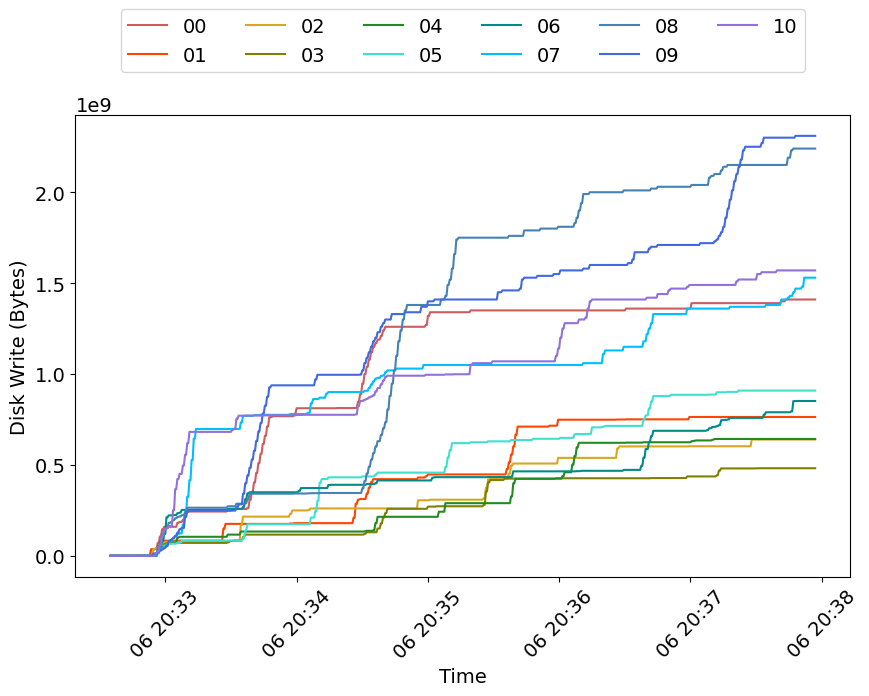
\includegraphics[width=\linewidth]{figures/ring/blk_write.png}
\caption{Ring topology -- amount of bytes written to disk}
\end{figure}
\begin{figure}[H]
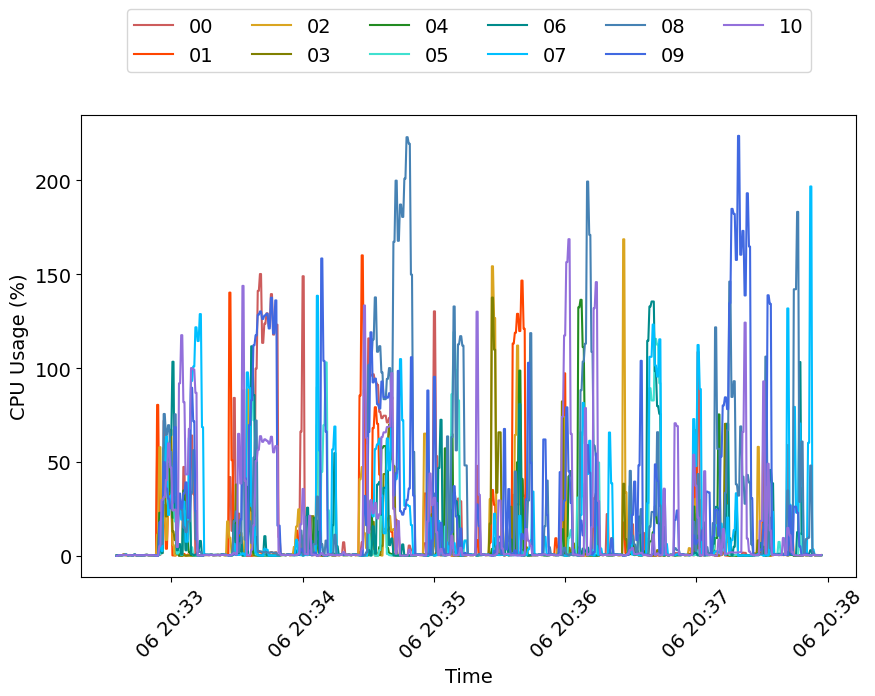
\includegraphics[width=\linewidth]{figures/ring/cpu_usage.png}
\caption{Ring topology -- CPU usage}
\end{figure}
\begin{figure}[H]
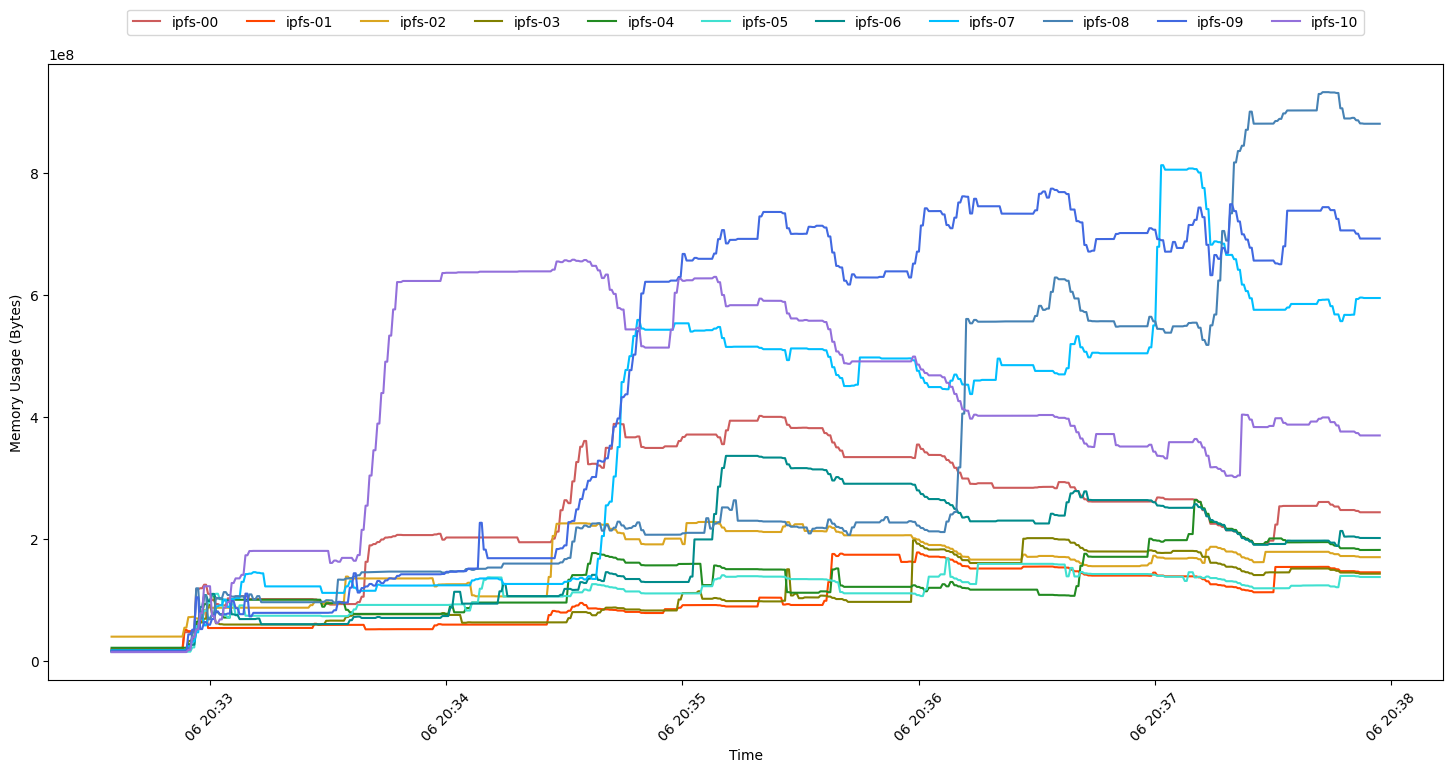
\includegraphics[width=\linewidth]{figures/ring/mem_usage.png}
\caption{Ring topology -- memory usage}
\end{figure}
\begin{figure}[H]
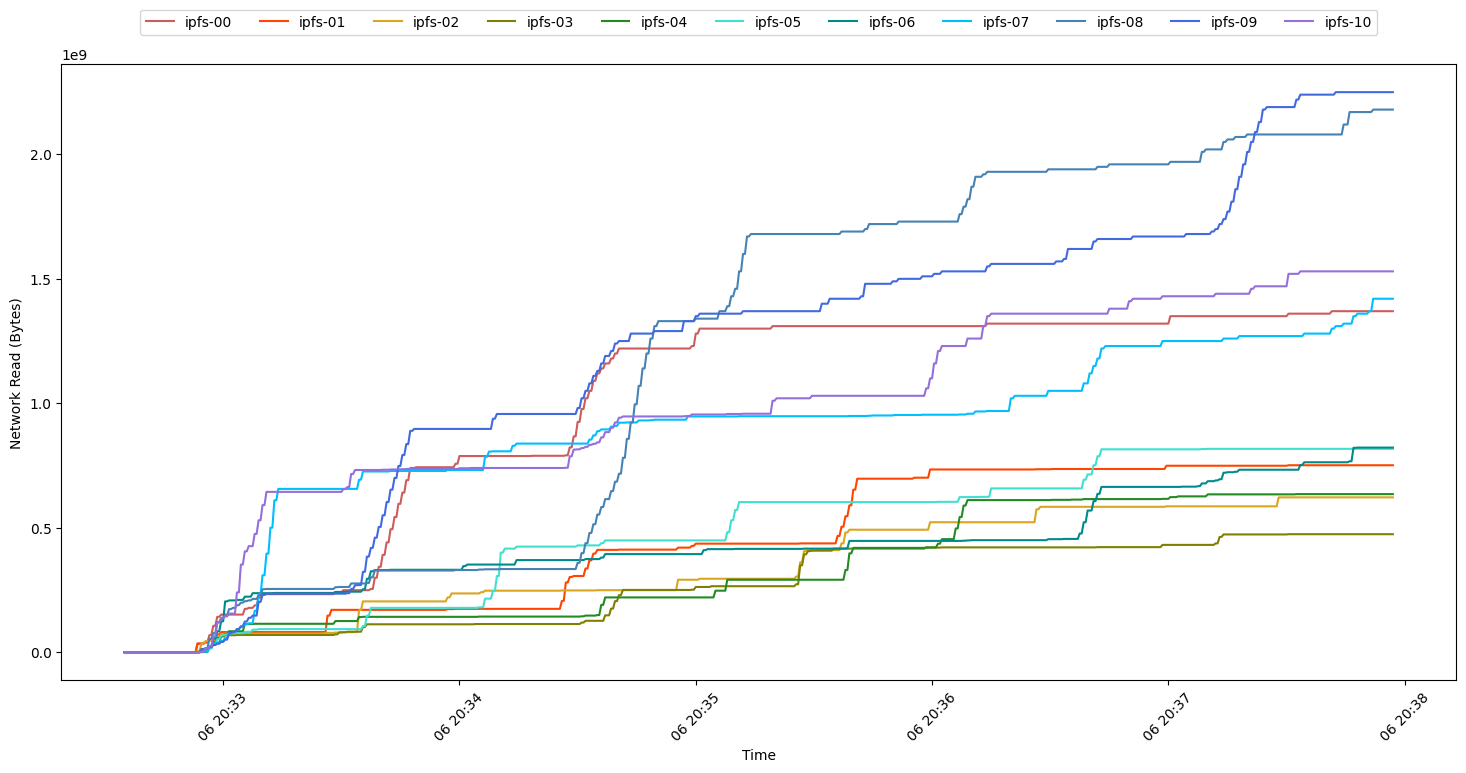
\includegraphics[width=\linewidth]{figures/ring/net_read.png}
\caption{Ring topology -- amount of bytes received over network}
\end{figure}
\begin{figure}[H]
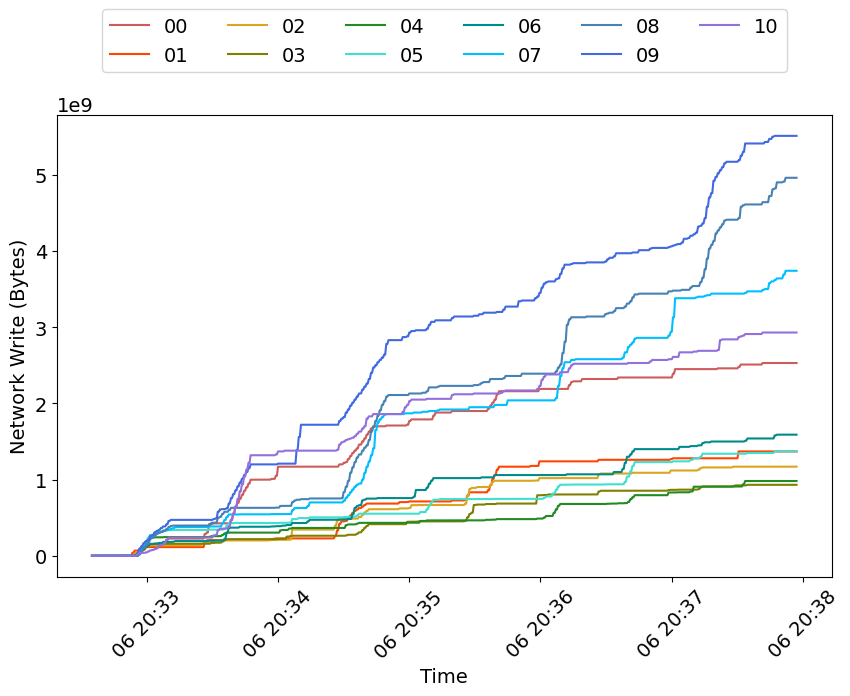
\includegraphics[width=\linewidth]{figures/ring/net_write.png}
\caption{Ring topology -- amount of bytes transmitted over network}
\end{figure}


\subsection{\textcolor{red}{Case 3: Grid Topology}}

\begin{figure}[H]
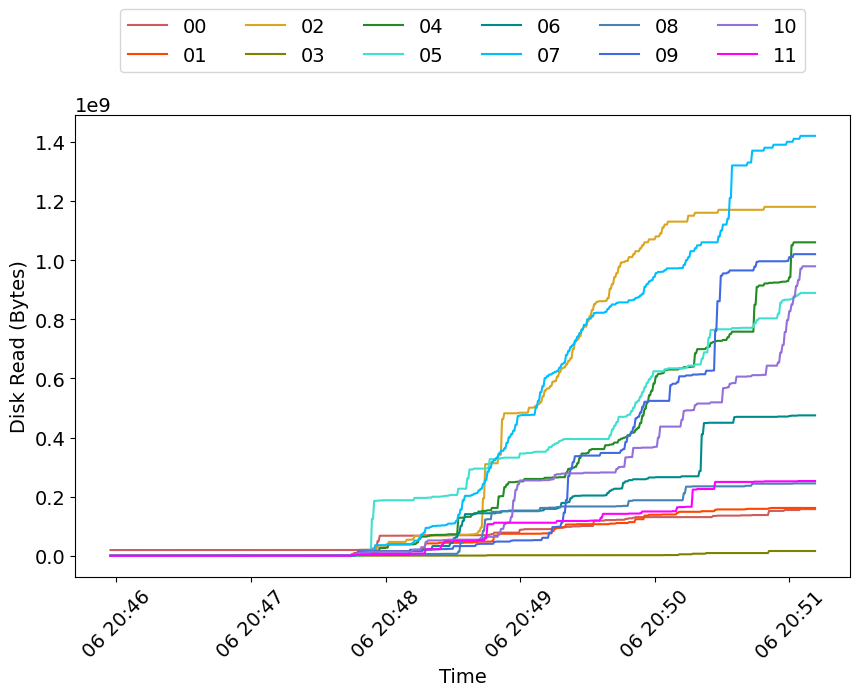
\includegraphics[width=\linewidth]{figures/grid/blk_read.png}
\caption{Grid topology -- amount of bytes read from disk}
\end{figure}
\begin{figure}[H]
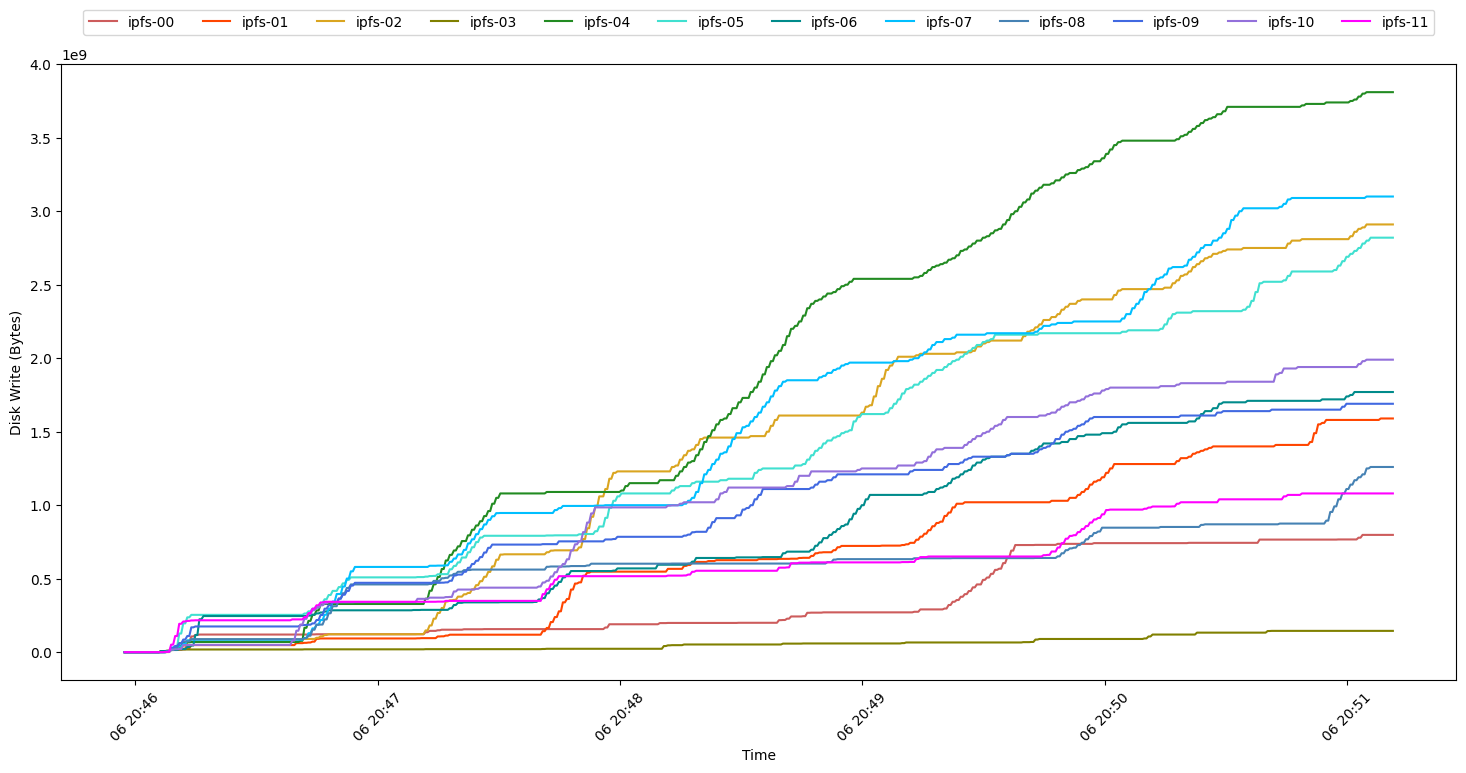
\includegraphics[width=\linewidth]{figures/grid/blk_write.png}
\caption{Grid topology -- amount of bytes written to disk}
\end{figure}
\begin{figure}[H]
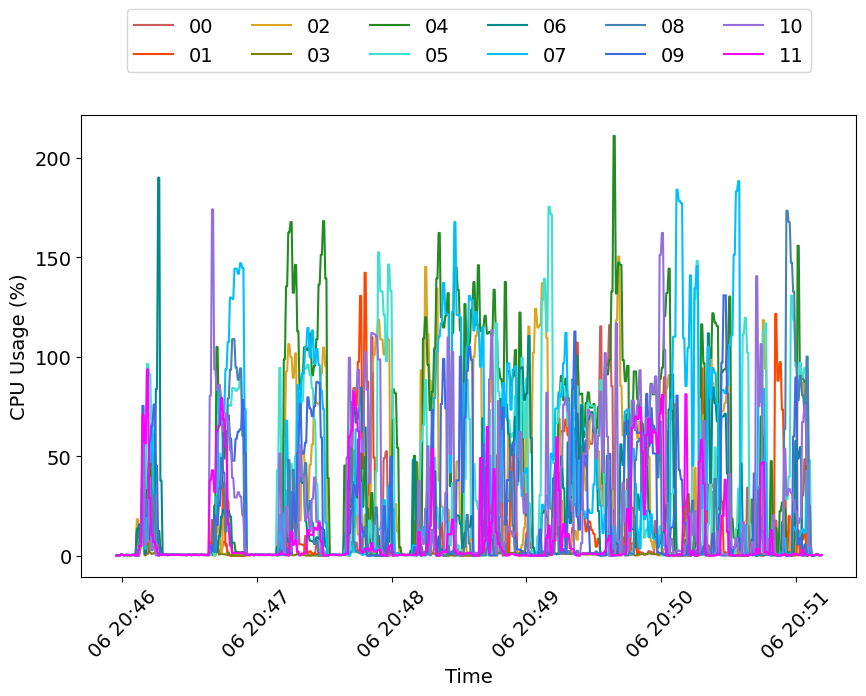
\includegraphics[width=\linewidth]{figures/grid/cpu_usage.png}
\caption{Grid topology -- CPU usage}
\end{figure}
\begin{figure}[H]
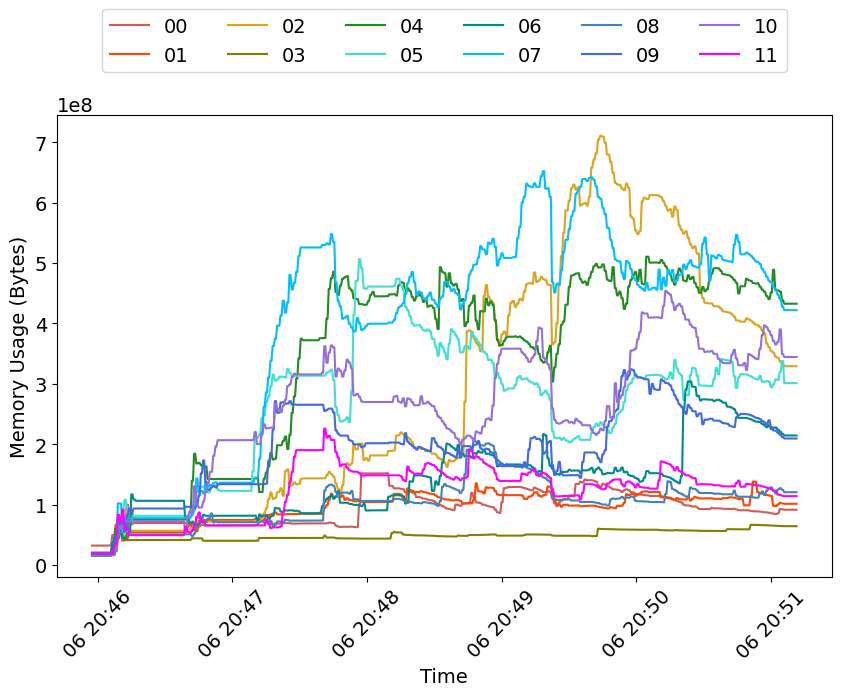
\includegraphics[width=\linewidth]{figures/grid/mem_usage.png}
\caption{Grid topology -- memory usage}
\end{figure}
\begin{figure}[H]
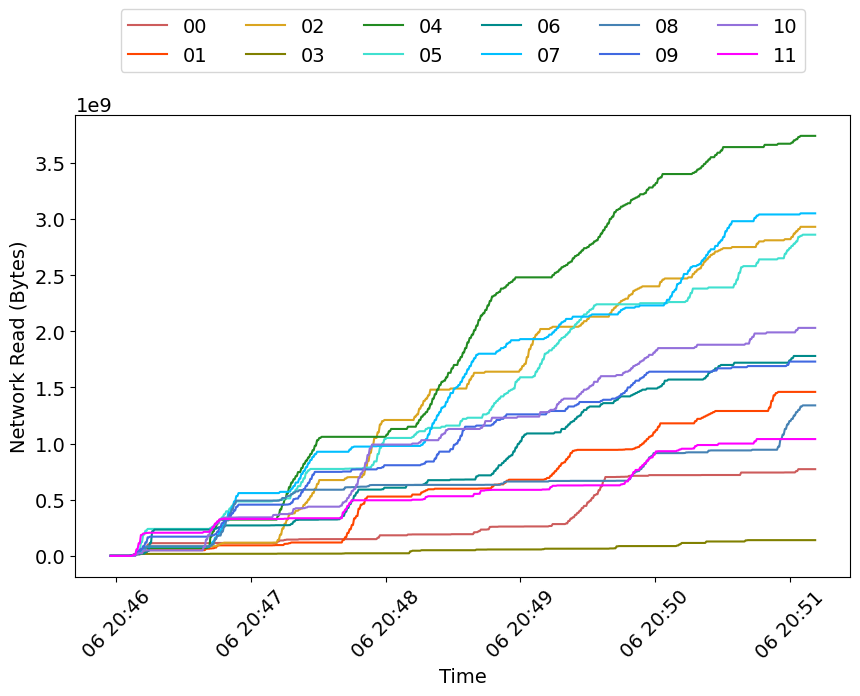
\includegraphics[width=\linewidth]{figures/grid/net_read.png}
\caption{Grid topology -- amount of bytes received over network}
\end{figure}
\begin{figure}[H]
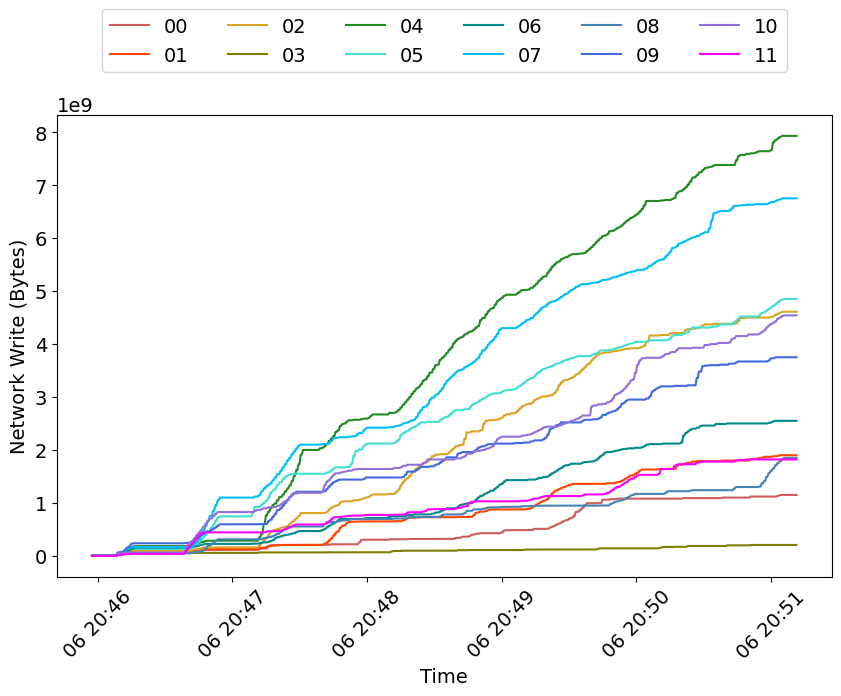
\includegraphics[width=\linewidth]{figures/grid/net_write.png}
\caption{Grid topology -- amount of bytes transmitted over network}
\end{figure}


\subsection{\textcolor{red}{Case 4: Random Graph Topology}}

\begin{figure}[H]
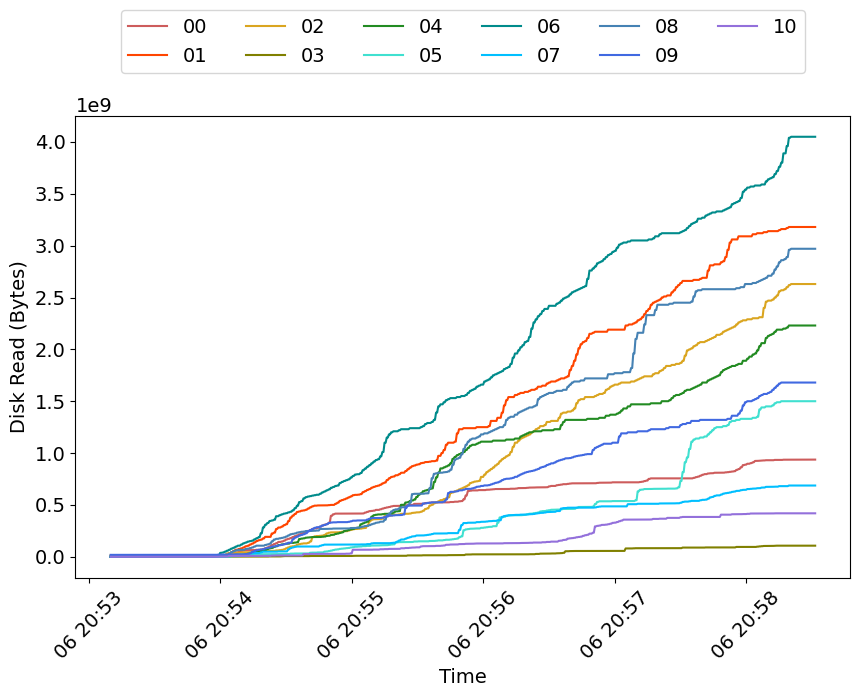
\includegraphics[width=\linewidth]{figures/graph-random/blk_read.png}
\caption{Random graph topology -- amount of bytes read from disk}
\end{figure}
\begin{figure}[H]
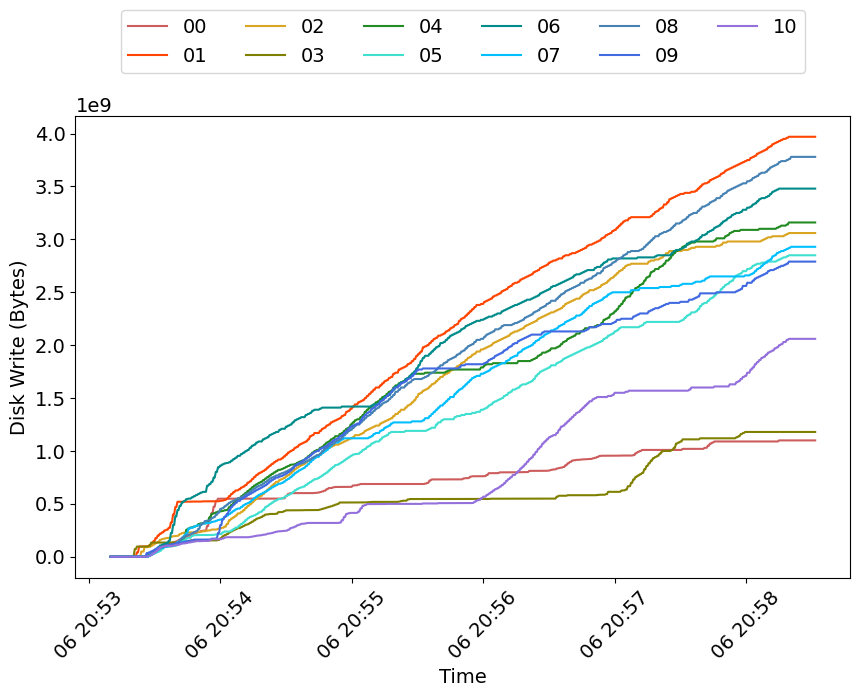
\includegraphics[width=\linewidth]{figures/graph-random/blk_write.png}
\caption{Random graph topology -- amount of bytes written to disk}
\end{figure}
\begin{figure}[H]
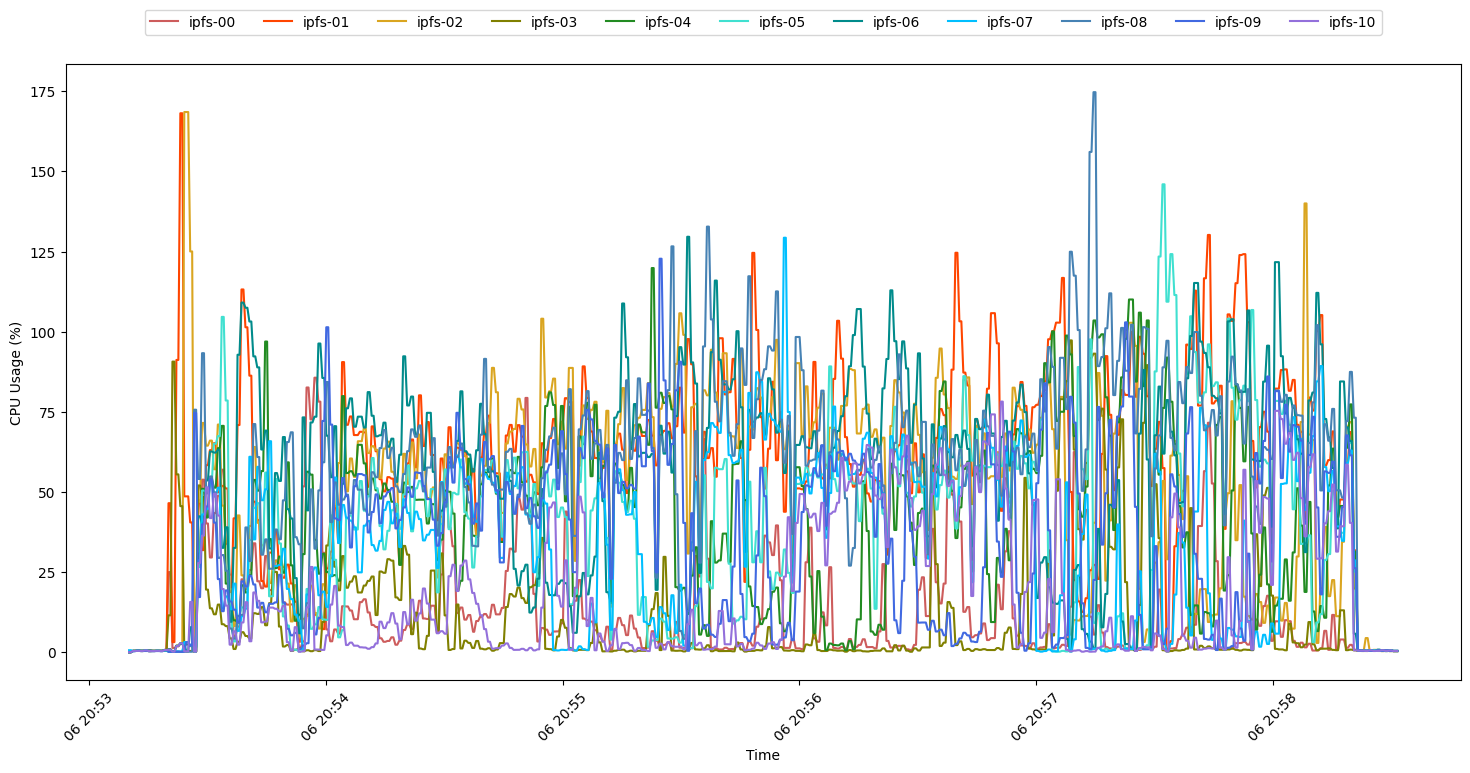
\includegraphics[width=\linewidth]{figures/graph-random/cpu_usage.png}
\caption{Random graph topology -- CPU usage}
\end{figure}
\begin{figure}[H]
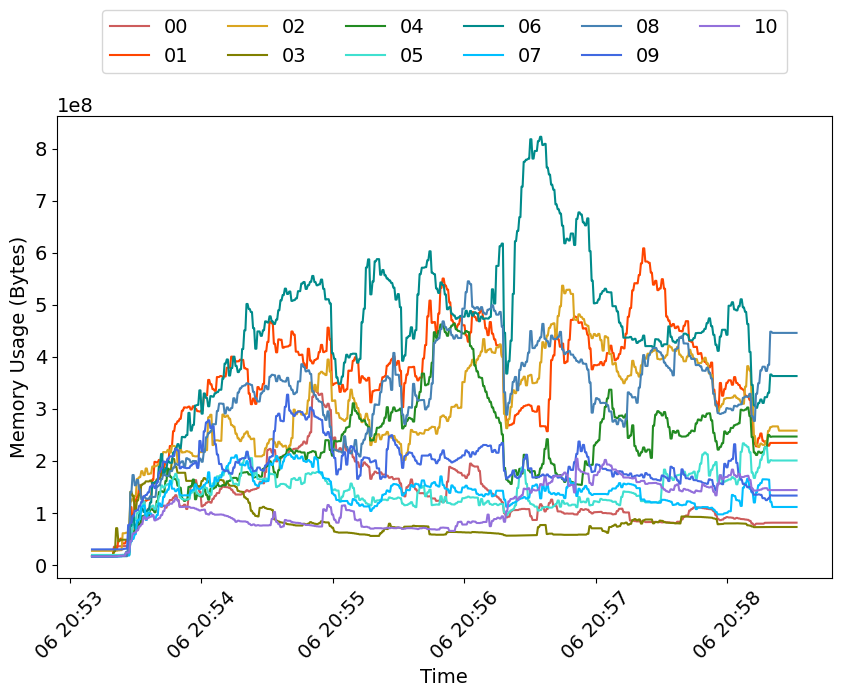
\includegraphics[width=\linewidth]{figures/graph-random/mem_usage.png}
\caption{Random graph topology -- memory usage}
\end{figure}
\begin{figure}[H]
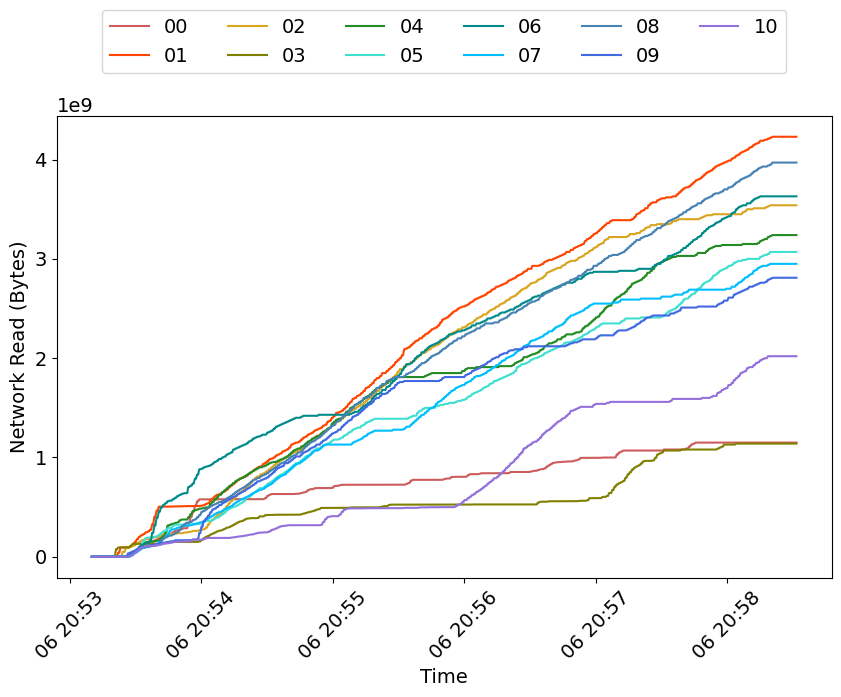
\includegraphics[width=\linewidth]{figures/graph-random/net_read.png}
\caption{Random graph topology -- amount of bytes received over network}
\end{figure}
\begin{figure}[H]
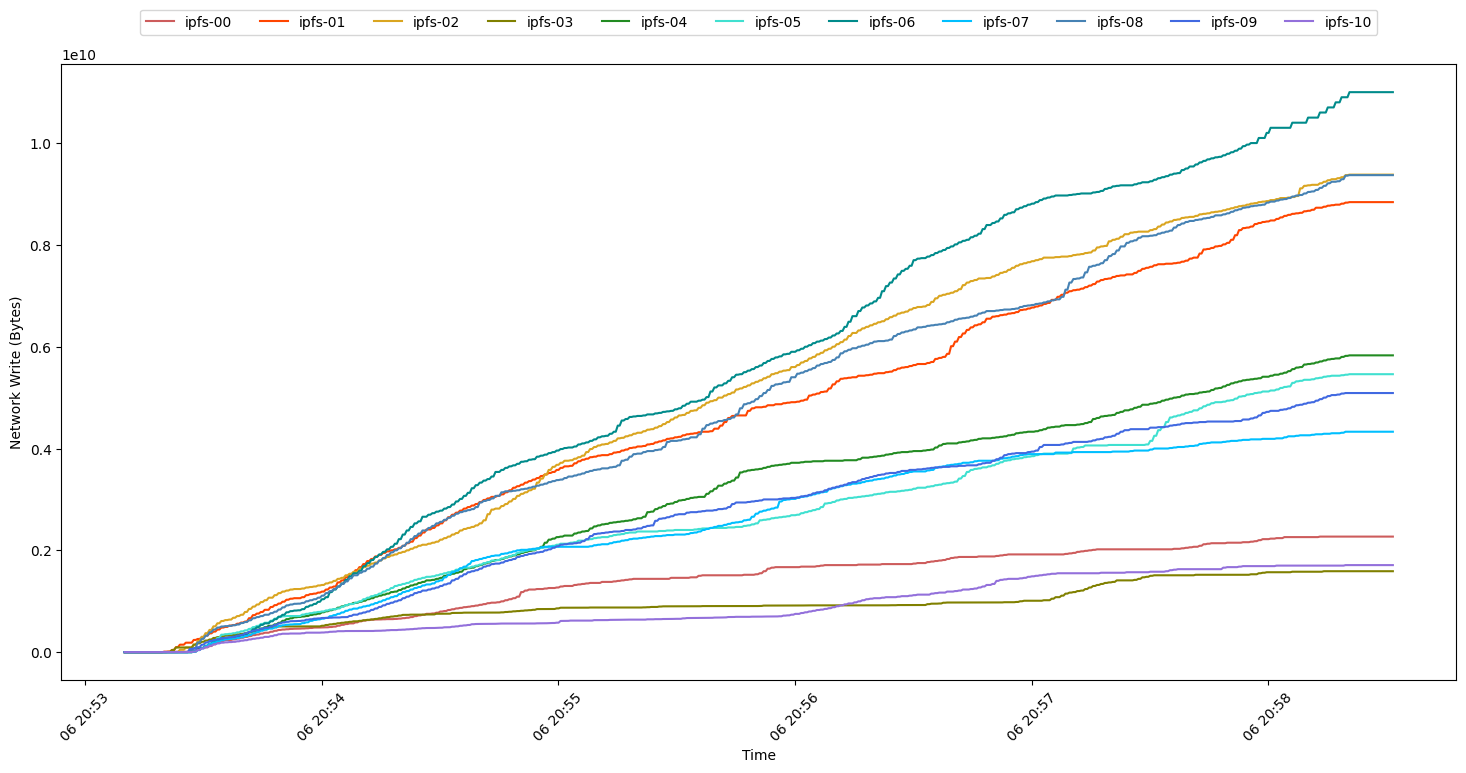
\includegraphics[width=\linewidth]{figures/graph-random/net_write.png}
\caption{Random graph topology -- amount of bytes transmitted over network}
\end{figure}


\subsection{\textcolor{red}{Case 5: Complete Graph Topology}}

\begin{figure}[H]
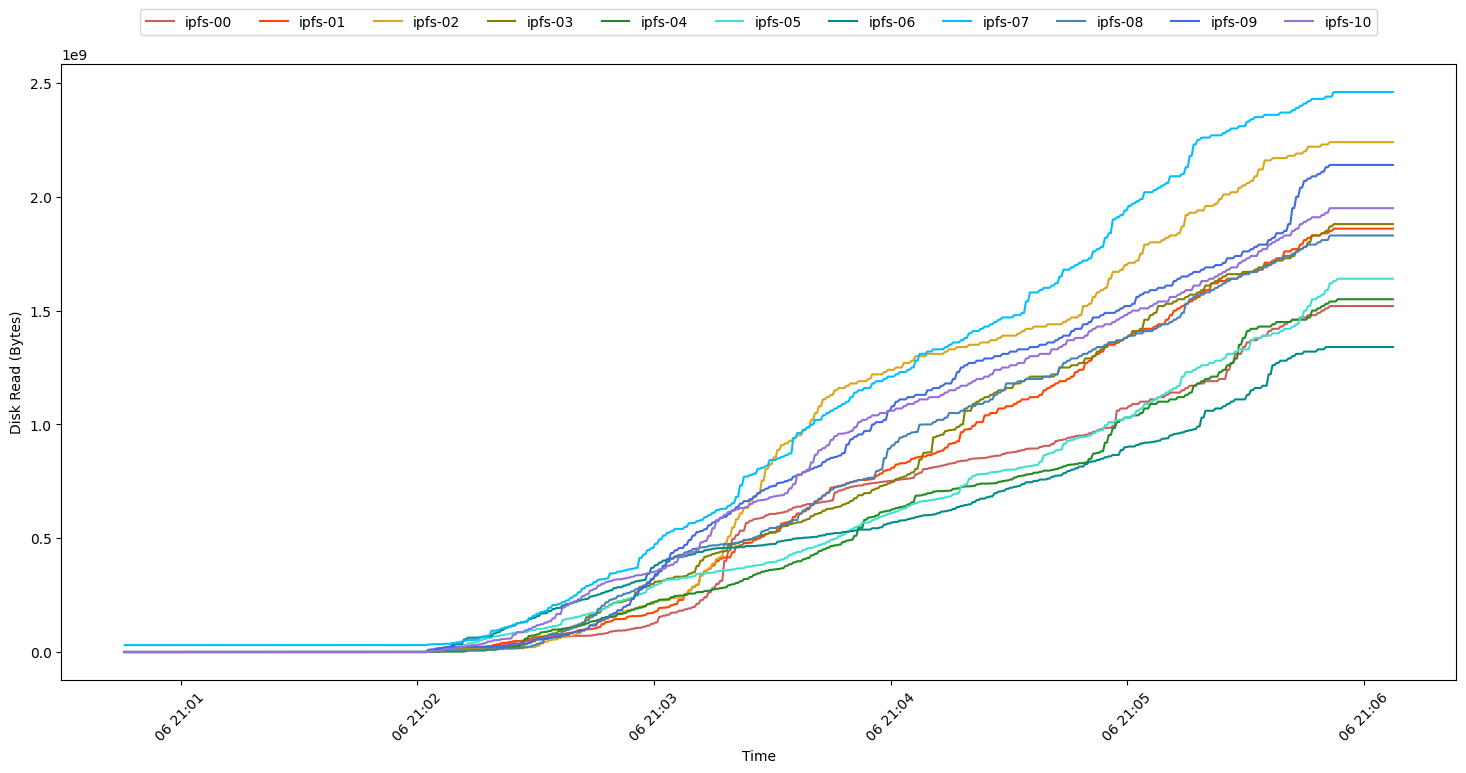
\includegraphics[width=\linewidth]{figures/graph-complete/blk_read.png}
\caption{Complete graph topology -- amount of bytes read from disk}
\end{figure}
\begin{figure}[H]
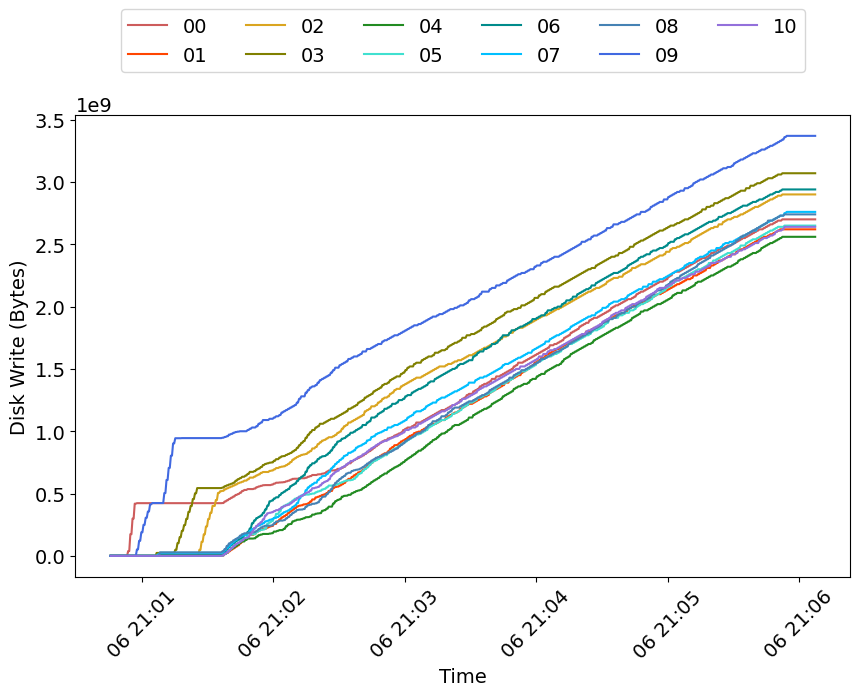
\includegraphics[width=\linewidth]{figures/graph-complete/blk_write.png}
\caption{Complete graph topology -- amount of bytes written to disk}
\end{figure}
\begin{figure}[H]
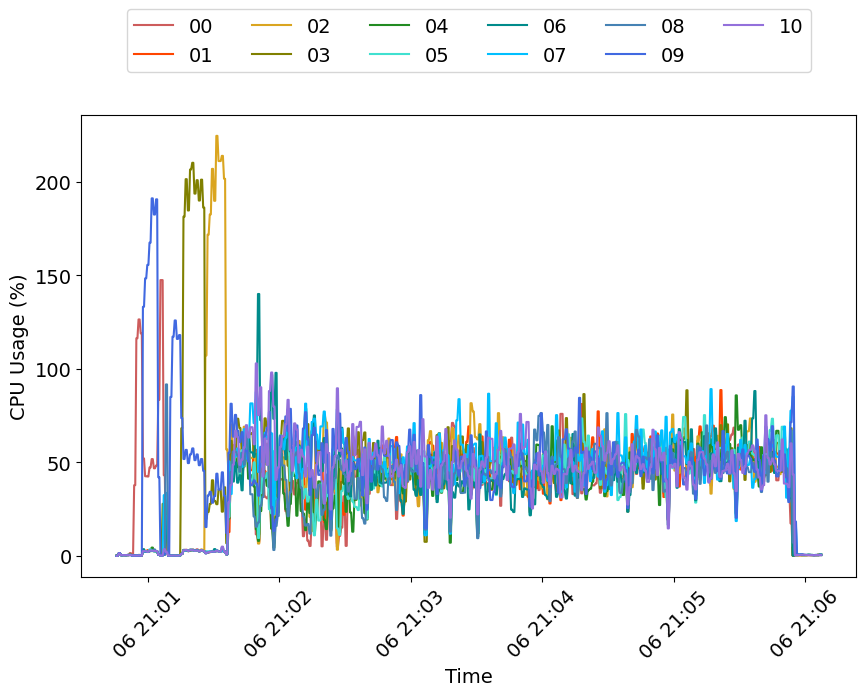
\includegraphics[width=\linewidth]{figures/graph-complete/cpu_usage.png}
\caption{Complete graph topology -- CPU usage}
\end{figure}
\begin{figure}[H]
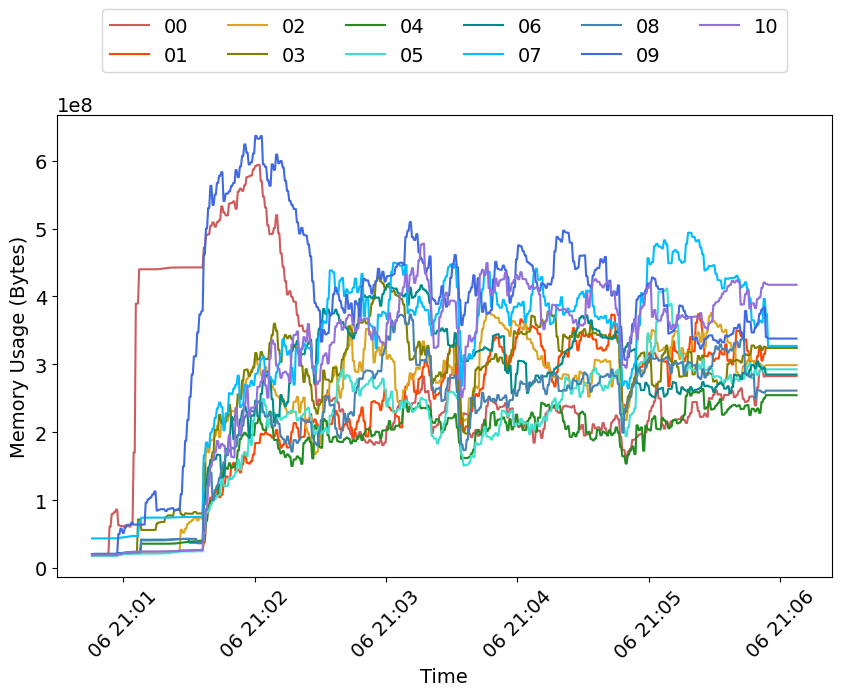
\includegraphics[width=\linewidth]{figures/graph-complete/mem_usage.png}
\caption{Complete graph topology -- memory usage}
\end{figure}
\begin{figure}[H]
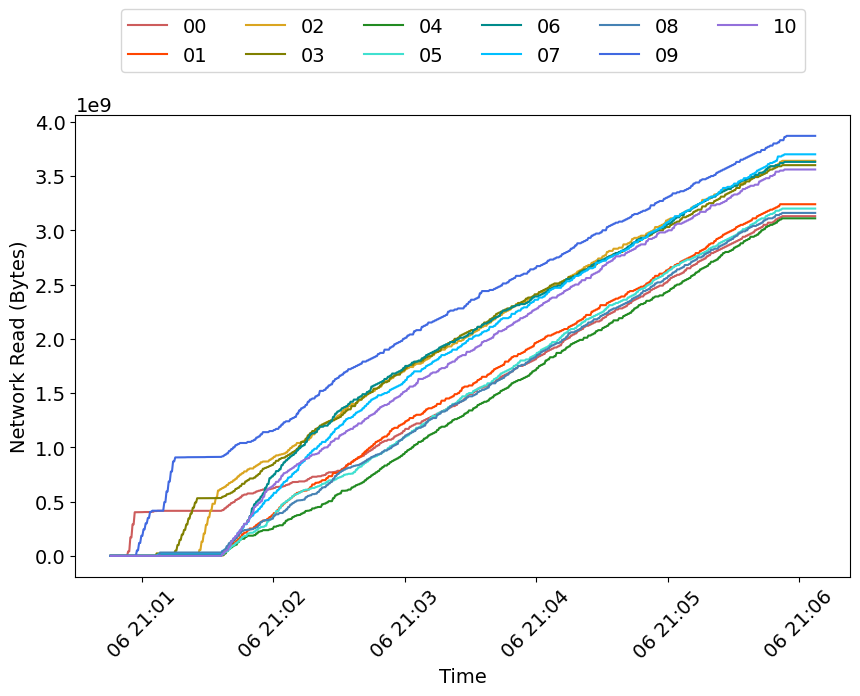
\includegraphics[width=\linewidth]{figures/graph-complete/net_read.png}
\caption{Complete graph topology -- amount of bytes received over network}
\end{figure}
\begin{figure}[H]
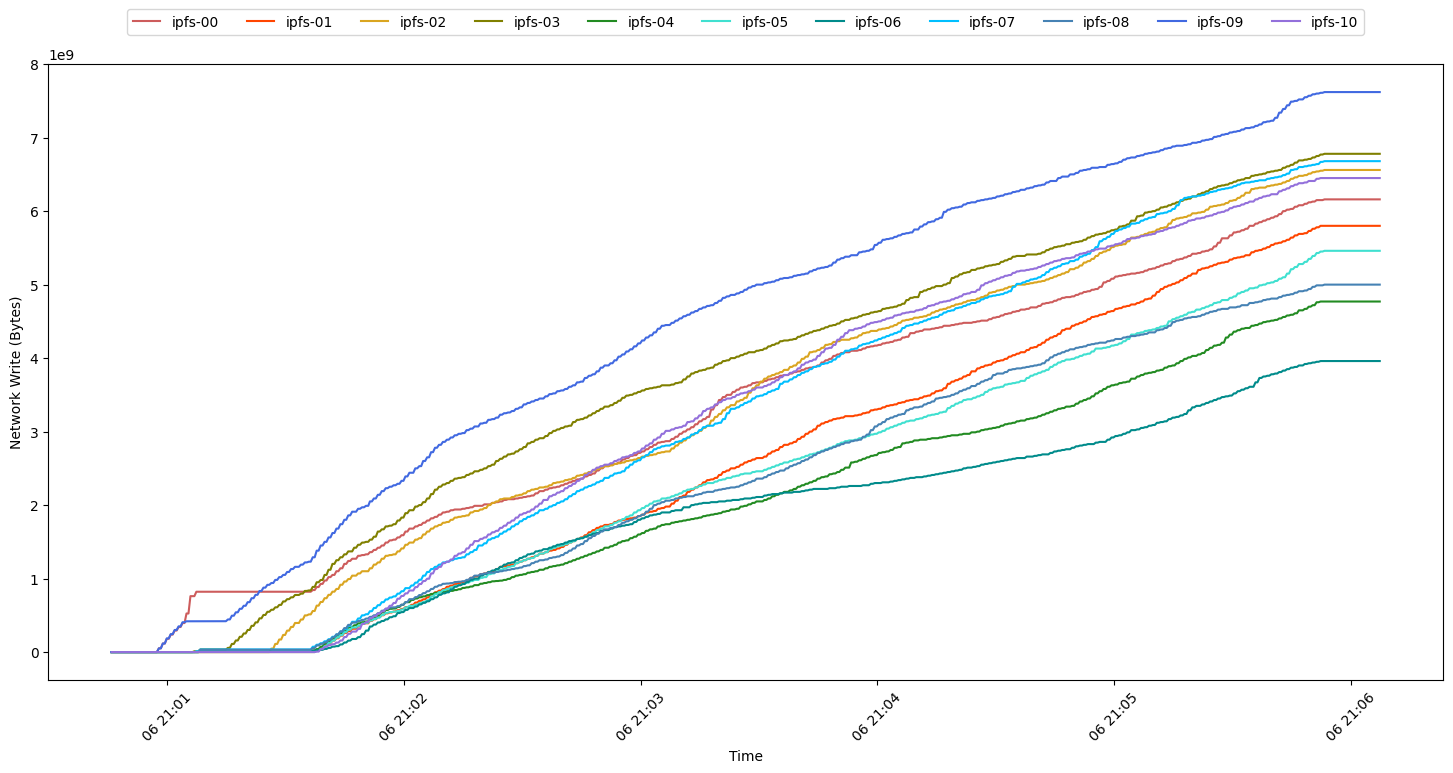
\includegraphics[width=\linewidth]{figures/graph-complete/net_write.png}
\caption{Complete graph topology -- amount of bytes transmitted over network}
\end{figure}


\subsection{\textcolor{red}{Conclusion}}
...


\end{document}
